% !TEX root = thesis-ex.tex
Extreme conditions of temperature and pressure like those in relativistic heavy ion collisions lead to the formation of the Quark Gluon Plasma \cite{SHURYAK198071}. It is believed to have filled the early universe a few microseconds after the Big Bang and might be present in the cores of extremely compact objects like neutron stars \cite{PhysRevLett.34.1353, Linde_1979}. The phase transition between the free quarks and gluons within the QGP and the confined quarks and gluons within hadrons can be seen in Figure~\ref{fig:qcd_phase}.  

\begin{figure}[htbp]
\begin{center}
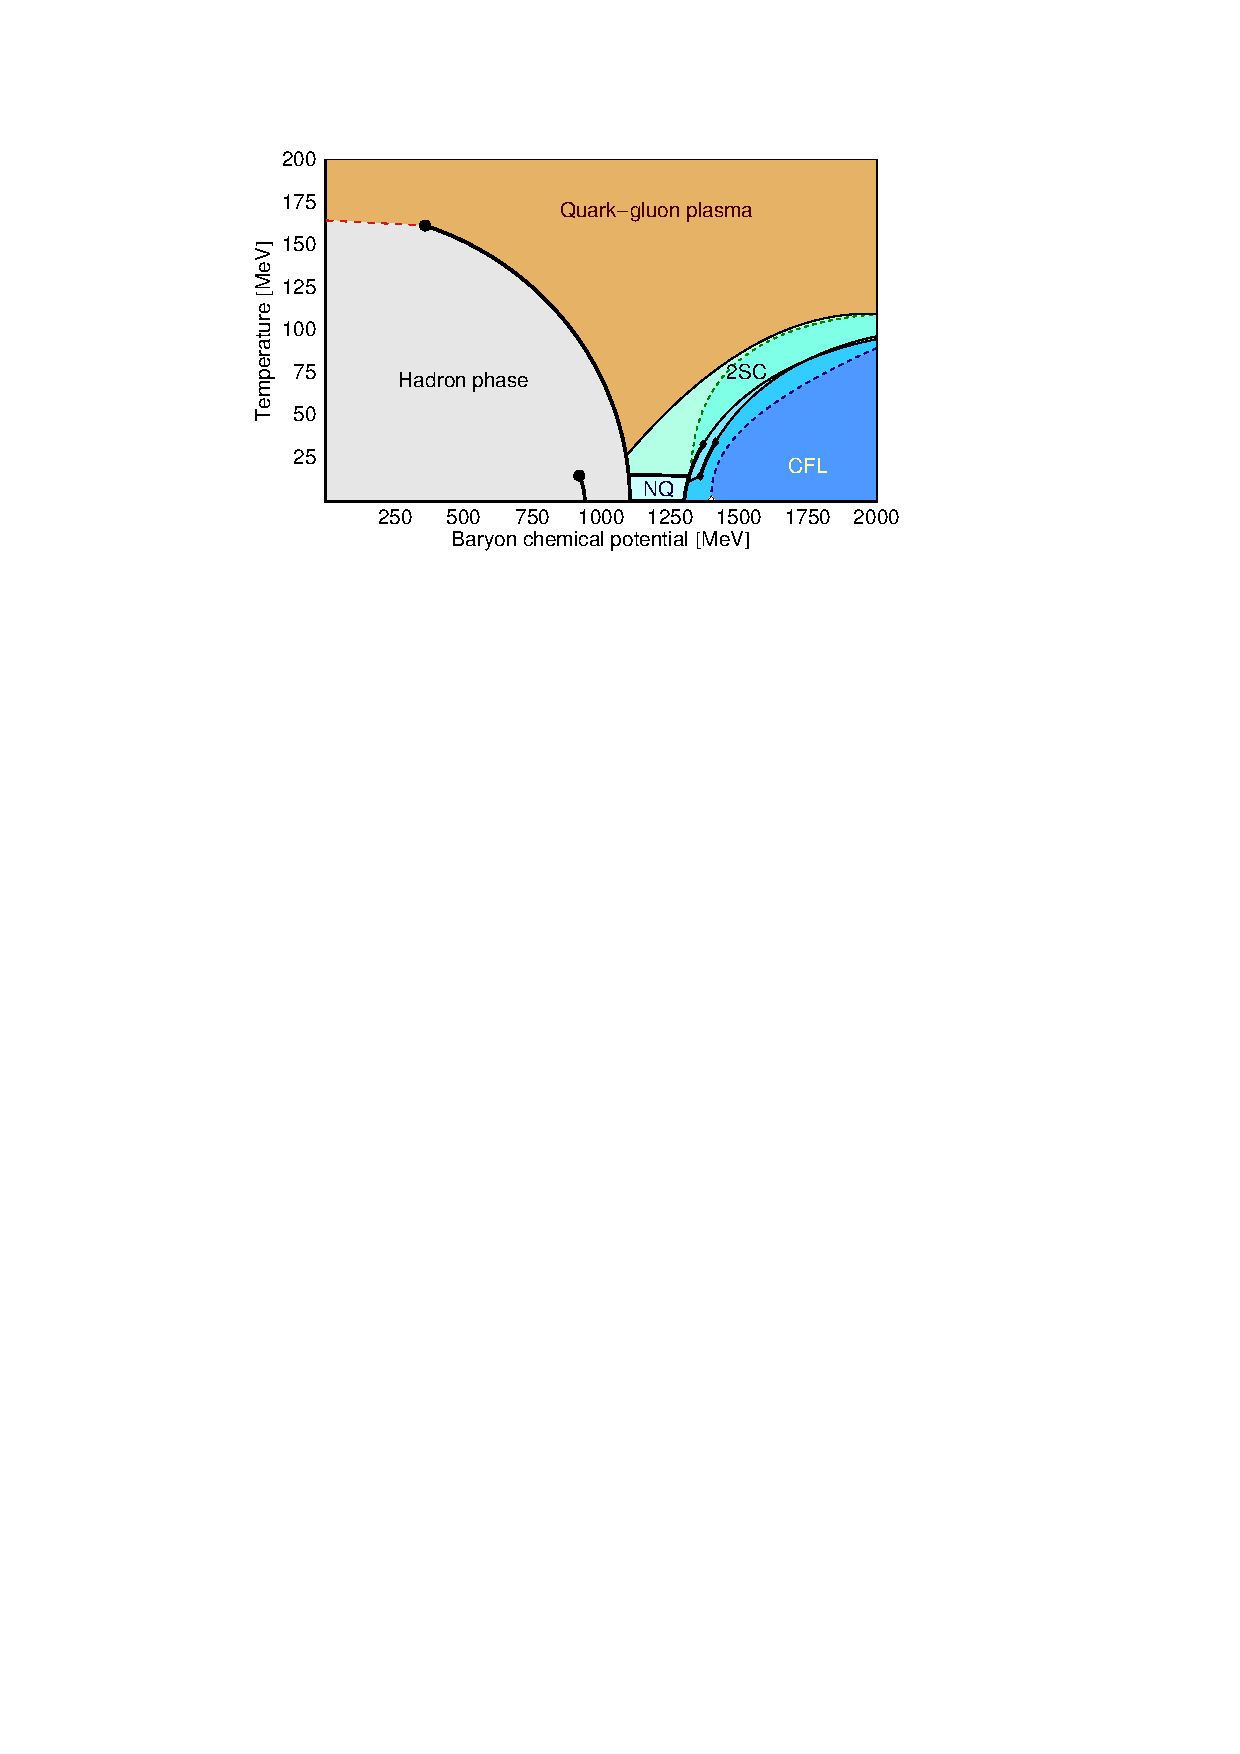
\includegraphics[width=0.85\textwidth]{figures/theory/qcd_phase}
\caption{The QCD phase diagram of nuclear matter. Figure from from Reference~\cite{PhysRevD.72.034004}. }
\label{fig:qcd_phase}
\end{center}
\end{figure}

This state of matter exists for 1-10 fm/c, depending on the collision energy, above $\lambda_{\mathrm{QCD}} = 200$ MeV, the fundamental energy scale in QCD. Thermal photons from the QGP reveal that it reaches temperatures of 300--600 MeV in central collisions at 200 GeV \cite{PhysRevLett.104.132301} and 2.76 TeV \cite{2016235}, showing very little collision energy dependence. Further, the chemical freeze-out temperature was found to be 160 MeV via measurements of ratios of final state hadrons containing the light $u, d$ quarks \cite{Fodor_2004, ADAMS2005102, PhysRevC.93.024917} with the thermal freeze-out being 100--150 MeV \cite{PhysRevC.69.024904, PhysRevC.72.014908, PhysRevC.75.024910, PhysRevC.88.044910}. These measurements paint a picture of the QGP being formed early in the heavy ion collision. It has a non-uniform energy density and temperature determined by the 'colliding nuclei and collision energy. The QGP then cools and expands as described by relativistic hydrodynamics, and as its temperature falls below 160 MeV, it experiences a crossover phase transition and hadronizes. This system continues to cool and expand, until at 95 GeV there is a thermal freeze-out. 




%The QGP can be further characterized by comparing quarkonia production in heavy ion and \pp\ collisions. 

%Supposing that the interactions between quarks and gluons are negligible, their energy density can be written in terms of the temperature $T$ and quark chemical potential $\mu$ as:
%
%\begin{align}
%\varepsilon_g &= \frac{16 \pi^2}{30} T^4 \\
%\varepsilon_q+\varepsilon_{\bar{q}} &= 12 \left( \frac{7\pi^2}{120} T^4 + \frac{1}{4}\mu^2 T^2 + \frac{1}{8\pi^2} \mu^4 \right)
%\end{align}
%Then, the thermodynamical quantities of pressure $P$, entropy density $s$ and baryon number density $\rho_B$ are given by:
%
%\begin{align}
%P = \frac{1}{3} \varepsilon, \qquad s = \left(\frac{\partial P}{\partial T}\right)_\mu, \qquad \rho_B = \frac{1}{3} \left( \frac{\partial P}{\partial \mu} \right)_T
%\end{align}
%
%Using the framework of the MIT Bag Model and assuming the QGP as an ideal gas with a bag constant $\mathcal{B}$ that parameterizes the vacuum pressure \cite{Muller1993, Yagi:2005yb}, the equation of state of the QGP can be written as
%
%\begin{align}
%\varepsilon &= \varepsilon_g(T, \mu) + \varepsilon_q(T, \mu) + \varepsilon_{\qbar} (T, \mu) + \mathcal{B} \\
%P &= P_g(T, \mu) + P_q(T, \mu) + P_{\qbar} (T, \mu) - \mathcal{B}
%\end{align}
%
%This model considers quarks and gluons to move freely inside a ``bag'' and postulates that a deconfined medium can be formed by compressing the bags together. Assuming a baryon free case with $\mu = 0$ and idealizing hadronic matter as a gas of non-interacting massless pions:
%
%\begin{align}
%\varepsilon_\pi = \frac{3\pi^2}{30} T^4, \qquad P_\pi = \frac{1}{3} \varepsilon_\pi
%\end{align}
%%%%%%%%%%%%%%%%%%%%%%%%%%%%

The QGP was initially thought to be a weakly coupled parton gas because of asymptotic freedom from QCD. The highly energetic collisions such as those at the LHC would imply a weak interaction between the quarks and gluons that make up the plasma. This would result in rare scatterings between the constituents of the gas and wash out any spatial anisotropies based on the collision geometry. On the other hand, a strong coupling within the QGP would result in the pressure gradients in the medium being driven by hydrodynamics and spatial anisotropies would be transformed to momentum anisotropies in the particles produced as shown in Figure~\ref{fig:overlap}. In this picture, the non-uniform structure of the colliding nuclei would cause a momentum anisotropy that would be further enhanced when looking at collisions that are less central and do not have perfect overlap between the colliding nuclei. These observations were seen in azimuthal correlation measurements implying that the medium is indeed strongly coupled \cite{Aaboud:2018ves, PhysRevLett.91.182301, Sirunyan:2017fts, PhysRevLett.116.132302}. 

\begin{figure}[htbp]
\begin{center}
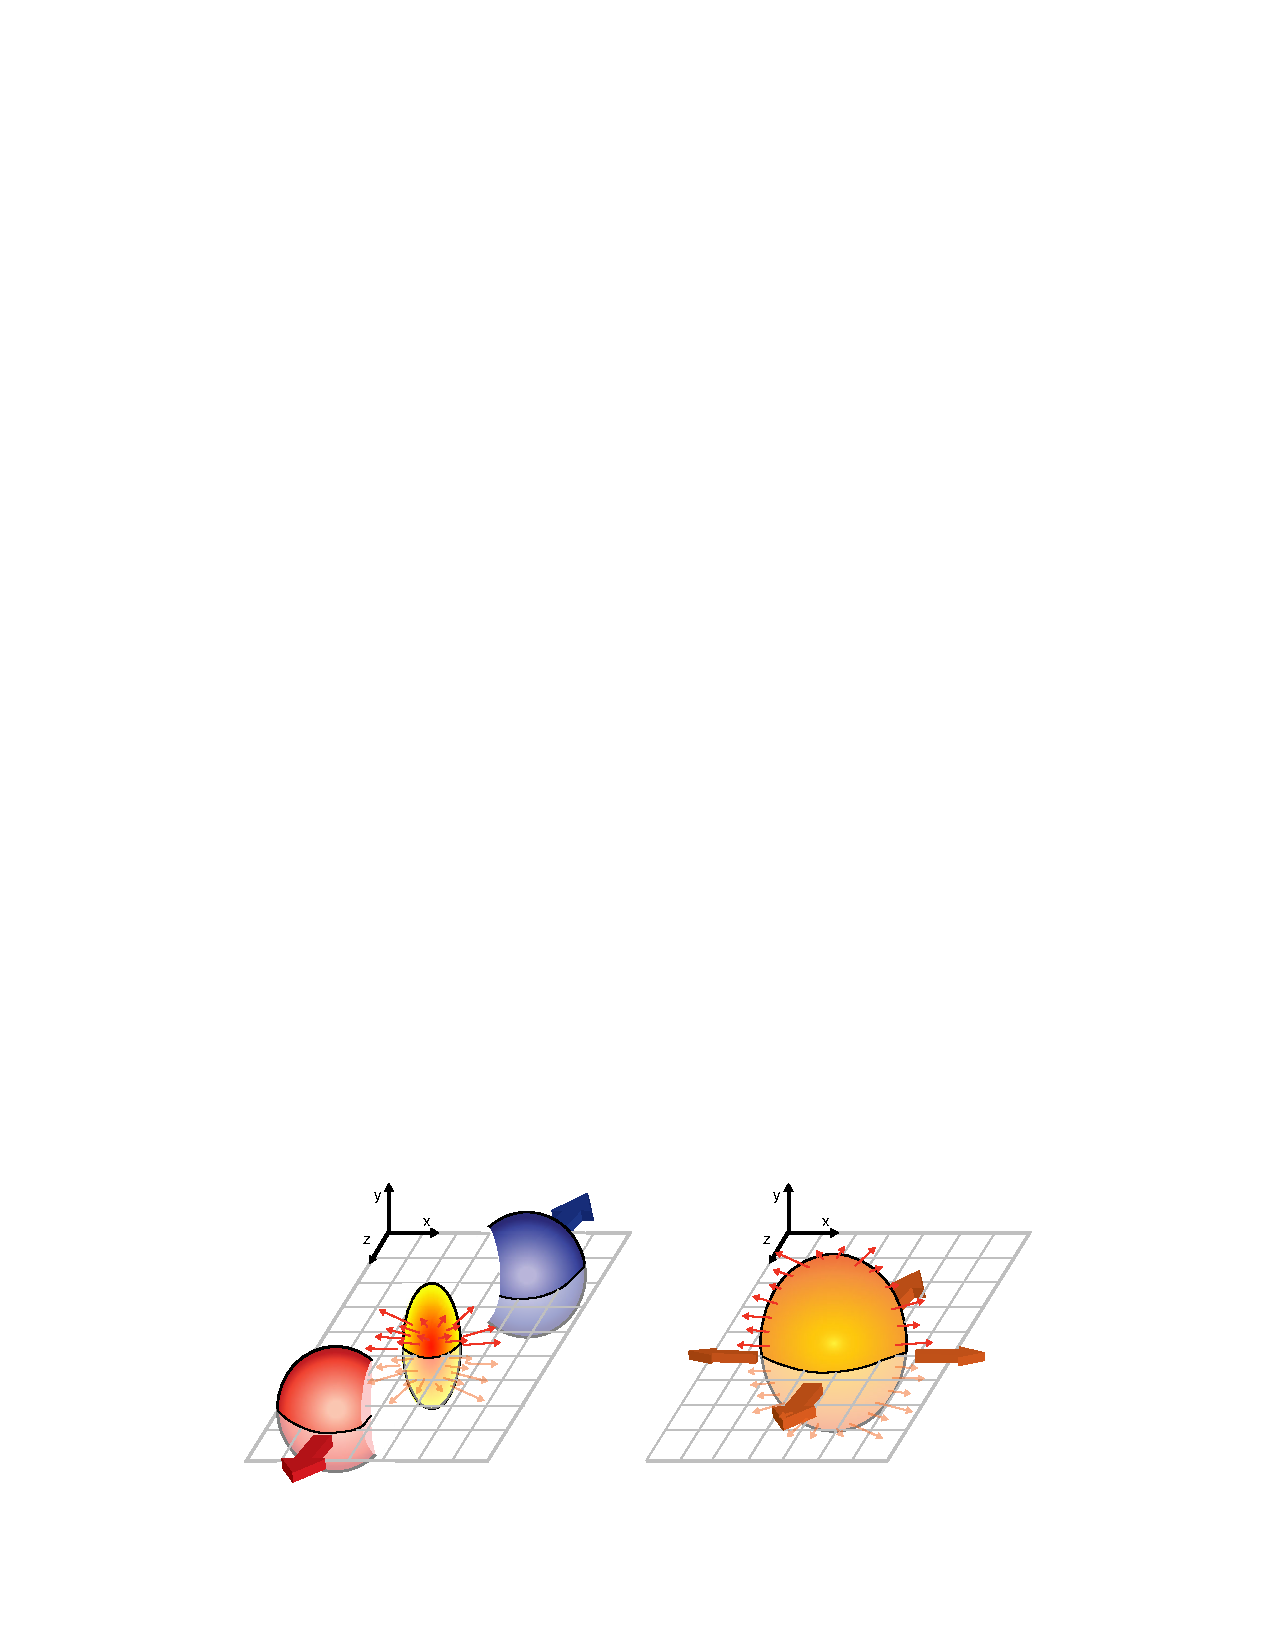
\includegraphics[width=0.85\textwidth]{figures/theory/overlap}
\caption{Schematic diagrams of the initial overlap region (left) and the final spatial anisotropy generated (right). Taken from \cite{RevModPhys.90.025005}.}
\label{fig:overlap}
\end{center}
\end{figure}

%At the peak energy density of the collision, the system cannot be described at the level of hadrons, and has to be described in terms of quarks and gluons. The initial anisotropic energy density being reflected in the azimuthal variation of particle production implies a strongly coupled medium that expands hydrodynamically, with a faster expansion in the direction of larger gradients and hence resulting a momentum anisotropy. 

A Fourier Transform of the angular distribution of charged hadrons in the collision debris can quantify these momentum anisotropies and give the anisotropic flow coefficients $v_n$, defined as \cite{Poskanzer:1998yz}:

\begin{align}
\frac{d\bar{N}}{d\phi} = \frac{\bar{N}}{2\pi} \left( 1 + 2 \sum_{n=1}^{\infty} v_{n} \cos(n(\phi-\bar{\Psi}_n)) \right)
\end{align}

where $\phi$ is the angle in the transverse plane, $\bar{\Psi}_n$ are the event plane angles, and $\bar{N}$ is the average number of particles per event. Some of these coefficients are shown in Figure~\ref{fig:flow_coeff}. The measured anisotropies can be used to constrain the specific viscosity given by the ratio of viscosity to entropy density, $\eta / s$, and have shown that the QGP has a $\eta / s$ of near the theoretical minimum of $1/4\pi$ \cite{Heinz:2013th}.


\begin{figure}[htbp]
\begin{center}
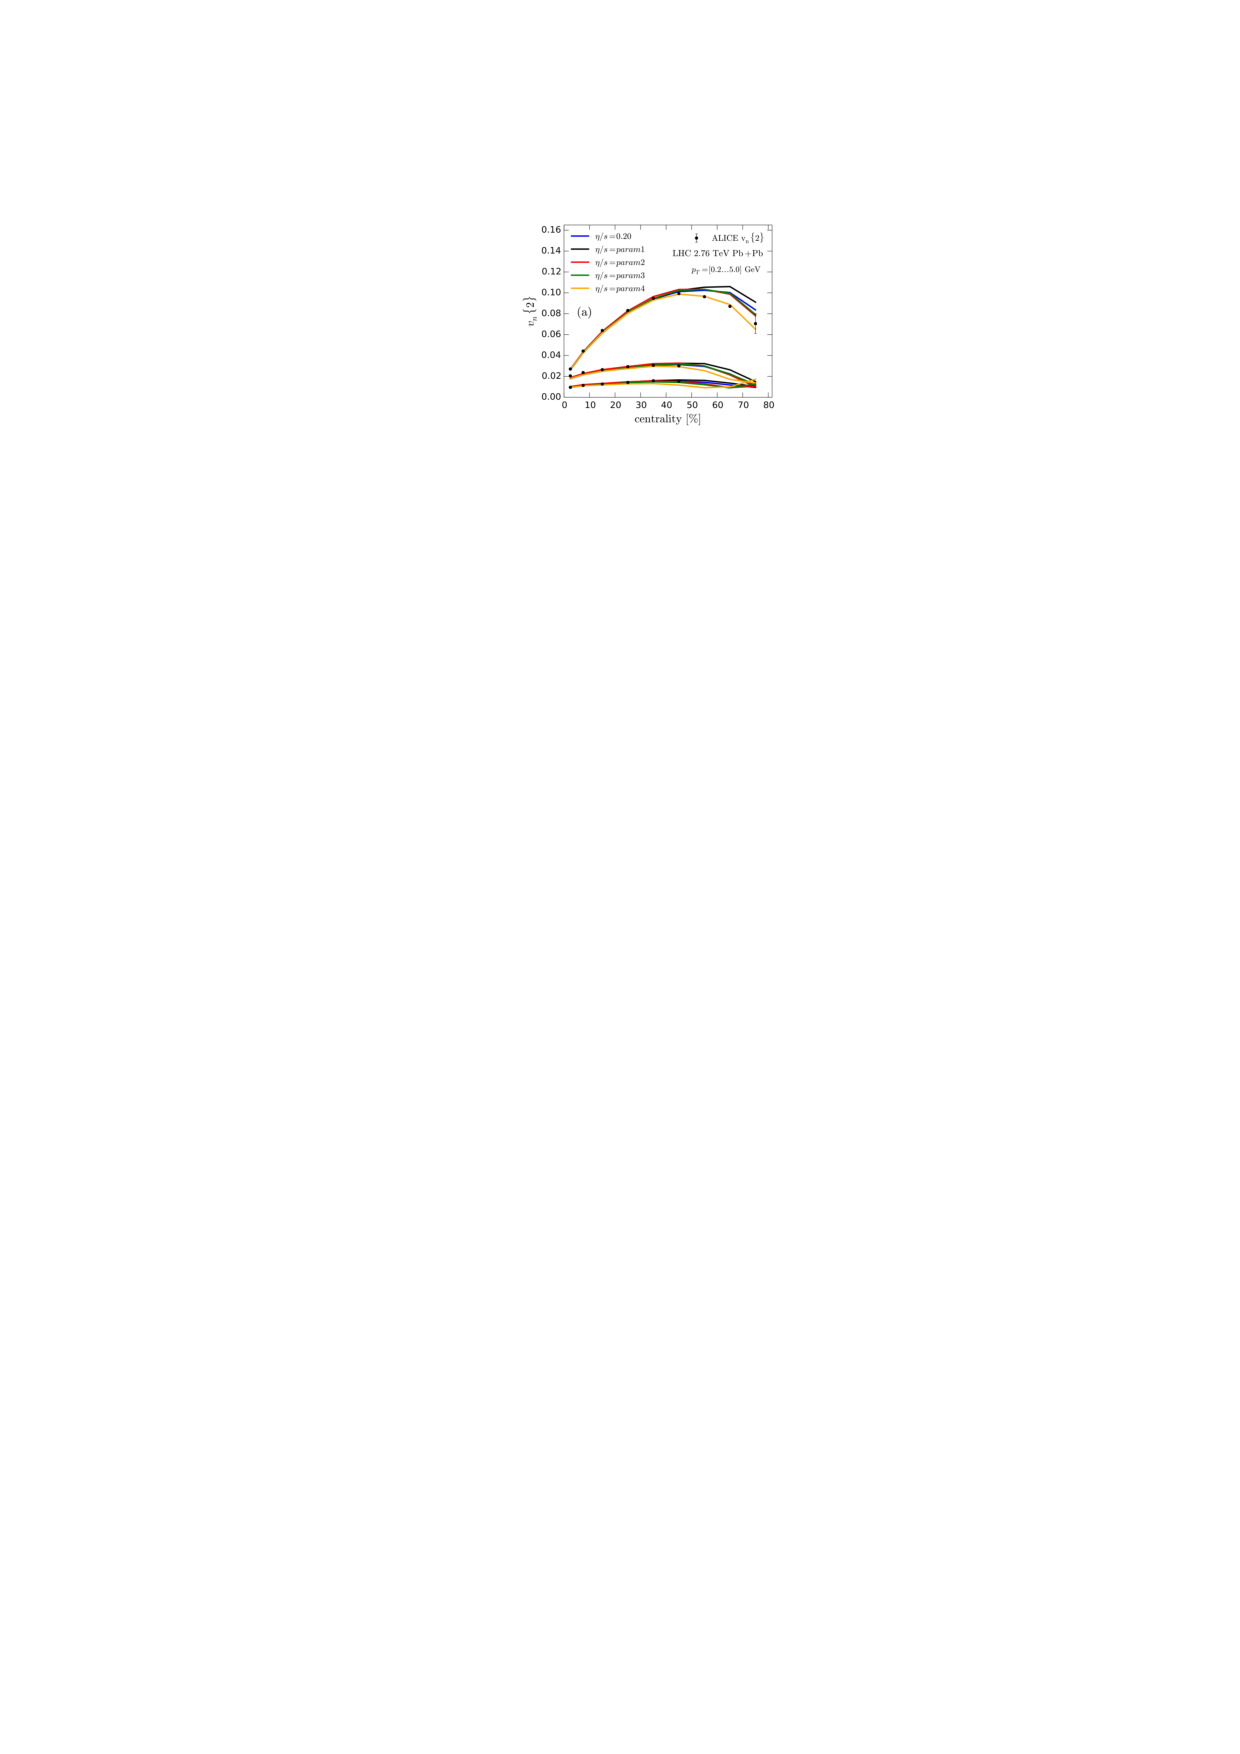
\includegraphics[width=0.65\textwidth]{figures/theory/flow_coefficients}
\caption{Comparison of a hydrodynamic model from \cite{Niemi:2015qia} to anisotropy measurements by ALICE \cite{ALICE:2011ab} for different parameterizations of $\eta / s $ and for different $v_n$, {\it{n}} = 2, 3, 4 from top to bottom, as a function of collision centrality.}
\label{fig:flow_coeff}
\end{center}
\end{figure}

The Bjorken energy density of the QGP can be derived using \cite{PhysRevD.27.140}:

\begin{align}
\varepsilon \geq \frac{d\Et/d\eta}{\tau_0 \pi R^2} = \frac{3}{2} \langle \Et/N \rangle \frac{d\Nch/d\eta}{\tau_0 \pi R^2}
\end{align}

where $d\Nch/d\eta$ is the number of charged particles produced per unity pseudorapidity, $d\Et/d\eta$ is the transverse energy per unit pseudorapidity, $\tau_0$ is the thermalization time, $R$ is the nuclear radius, and $\Et/N \approx 1$ GeV is the transverse energy per emitted particle. As shown in Figure~\ref{fig:energyDensity}, the energy density at the LHC was measured to be approximately 15 $\mathrm{GeV} / \mathrm{fm}^3$, much higher than the values measured at RHIC \cite{Adcox:2004mh, Krajcz_r_2011}.




\begin{figure}[htbp]
\begin{center}
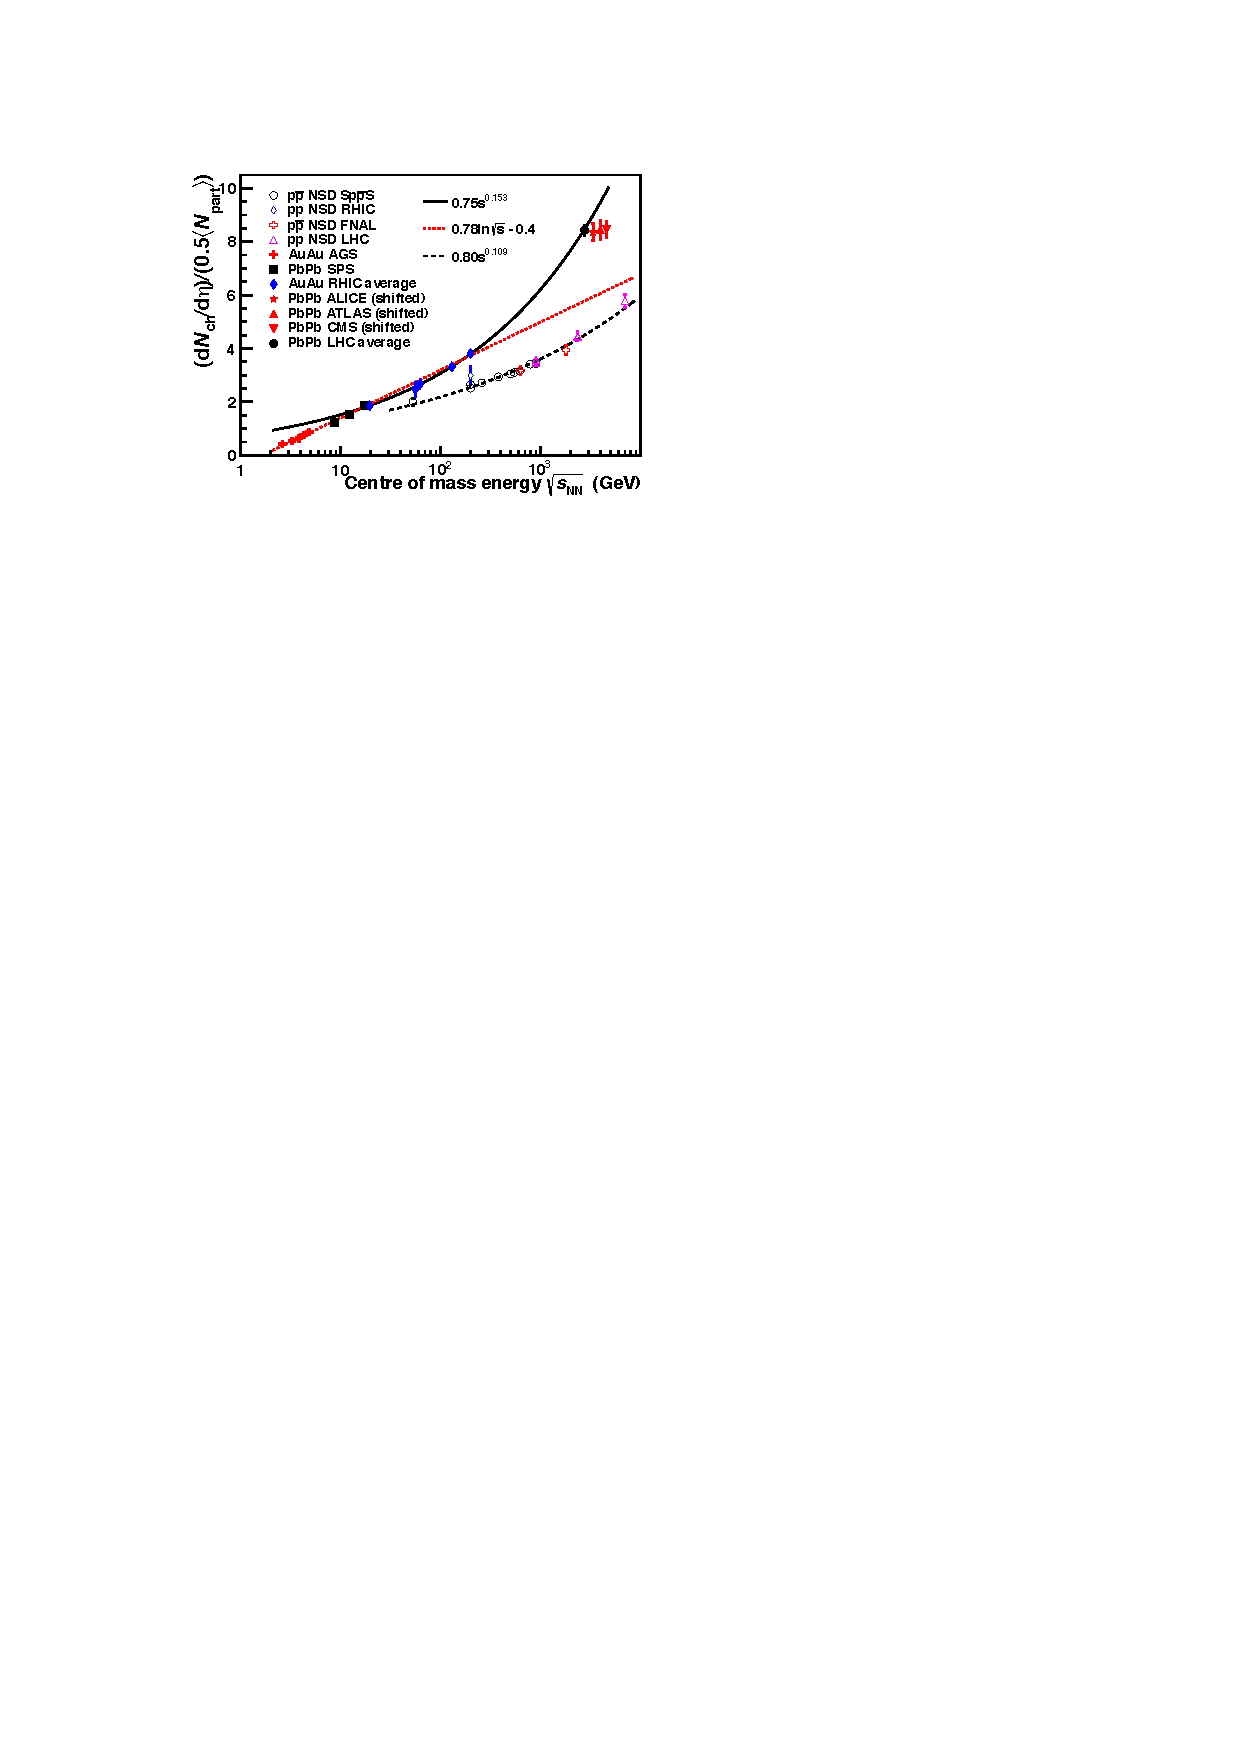
\includegraphics[width=0.65\textwidth]{figures/theory/energyDensity}
\caption{$d\Nch/d\eta$ per colliding nucleon pair as a function of collision energy in \pp\ and nucleus-nucleus collisions \cite{Muller:2012zq}. }
\label{fig:energyDensity}
\end{center}
\end{figure}






















